\subsection{Fubini and Tonelli Theorems}

\begin{theorem} \label{thm:tonelli-sigma-finite-product-measures} \hlt{Tonelli's Theorem for $\sigma$-Finite Products}\\
Let $(X,\mathcal M,\mu)$, $(Y,\mathcal N,\nu)$ be $\sigma$-finite, Let $Z\defeq X\times Y$, $\pi\defeq\mu\otimes\nu$.\\
Let $F:Z\to[0,+\infty]$ be $\mathcal M\otimes\mathcal N$-measurable. Put $I_F(x)\defeq\int_YF_x\,d\nu$ and $J_F(y)\defeq\int_XF^y\,d\mu$.
\begin{enumerate}[label=(\roman*)]
\setlength{\itemsep}{0pt}
\item $I_F$ is $\mathcal M$-measurable.
\item $J_F$ is $\mathcal N$-measurable.
\item $\int_XI_F\,d\mu=\int_ZF\,d\pi=\int_YJ_F\,d\nu$.
\end{enumerate}
\begin{proof} For $F=\mathbf{1}_E$, Proposition \ref{prop:section-measures-integrate-to-product-measure} gives the claims.\\
Finite linearity gives them for nonnegative simple $\Phi=\sum_{j=1}^na_j\mathbf{1}_{E_j}$. Choose simple $0\leq\Phi_n\uparrow F$.
\begin{enumerate}[label=(\roman*)]
\setlength{\itemsep}{0pt}
\item Since $I_{\Phi_n}$ is $\mathcal M$-measurable and $I_{\Phi_n}(x)=\int_Y(\Phi_n)_x\,d\nu\uparrow\int_YF_x\,d\nu=I_F(x)$, $I_F$ is $\mathcal M$-measurable.
\item Since $J_{\Phi_n}$ is $\mathcal N$-measurable and $J_{\Phi_n}(y)=\int_X(\Phi_n)^y\,d\mu\uparrow\int_XF^y\,d\mu=J_F(y)$, $J_F$ is $\mathcal N$-measurable.
\item From $\int_XI_{\Phi_n}\,d\mu=\int_Z\Phi_n\,d\pi=\int_YJ_{\Phi_n}\,d\nu$, MCT in $X$, $Z$, and $Y$ gives $\int_XI_F\,d\mu=\int_ZF\,d\pi=\int_YJ_F\,d\nu$.
\end{enumerate}
\hlt{Structural Commentary}: Approximate by nonnegative simple functions.\\
\hlt{Key Insight}: MCT passes sections and integrals together.
\end{proof}
\end{theorem}

\begin{theorem} \label{thm:fubini-sigma-finite-product-measures} \hlt{Fubini's Theorem for $\sigma$-Finite Products}\\
Let $(X,\mathcal{M},\mu)$ and $(Y,\mathcal{N},\nu)$ be $\sigma$-finite, $\pi\defeq\mu\otimes\nu$, and $F\in\mathscr{L}^1(\pi)$.
\begin{enumerate}[label=(\roman*)]
\setlength{\itemsep}{0pt}
\item $F_x\in\mathscr{L}^1(\nu)$ for $\mu$-a.e. $x$ and $F^y\in\mathscr{L}^1(\mu)$ for $\nu$-a.e. $y$.
\item With $f(x)\defeq\int_YF_x\,d\nu$ and $g(y)\defeq\int_XF^y\,d\mu$ on those full-measure sets, and $0$ elsewhere, $f\in\mathscr{L}^1(\mu)$, $g\in\mathscr{L}^1(\nu)$, and $\int_Xf\,d\mu=\int_ZF\,d\pi=\int_Yg\,d\nu$.
\end{enumerate}
\begin{proof}
\begin{enumerate}[label=(\roman*)]
\setlength{\itemsep}{0pt}
\item Tonelli on $\abs{F}$ gives $\int_X(\int_Y\abs{F_x}\,d\nu)d\mu=\int_Z\abs{F}\,d\pi=\int_Y(\int_X\abs{F^y}\,d\mu)d\nu<+\infty$, hence finite a.e.
\item Tonelli on $F^+$ and $F^-$ gives finite identities; subtract them to obtain $\int_Xf\,d\mu=\int_ZF\,d\pi=\int_Yg\,d\nu$.\\
Moreover $\abs{f}\leq\int_Y\abs{F_x}\,d\nu$ and $\abs{g}\leq\int_X\abs{F^y}\,d\mu$, so (i) gives $f,g\in\mathscr{L}^1$.
\end{enumerate}
\hlt{Structural Commentary}: Fubini is Tonelli plus subtraction.\\
\hlt{Key Insight}: $\int\abs{F}<+\infty$ makes the two nonnegative Tonelli identities finite enough to subtract.
\end{proof}
\end{theorem}

\begin{proposition} \label{prop:product-borel-and-measurable-building-blocks} \hlt{Product Borel and Measurable Building Blocks}\\
The following hold.
\begin{enumerate}[label=(\roman*)]
\setlength{\itemsep}{0pt}
\item $\mathcal{B}(\R)\otimes\mathcal{B}(\R)=\mathcal{B}(\R^2)$.
\item If $f:X\to\R$ is $\mathcal{M}$-measurable and $g:Y\to\R$ is $\mathcal{N}$-measurable,\\
then $(x,y)\mapsto f(x)g(y)$ is $\mathcal{M}\otimes\mathcal{N}$-measurable.
\item If $u:\R\to\R$ is Borel measurable, then $(x,y)\mapsto u(x-y)$ is $\mathcal{B}(\R)\otimes\mathcal{B}(\R)$-measurable.
\end{enumerate}
\begin{proof}
\begin{enumerate}[label=(\roman*)]
\setlength{\itemsep}{0pt}
\item Open rectangles give $\mathcal{B}(\R)\otimes\mathcal{B}(\R)\subseteq\mathcal{B}(\R^2)$.\\
Conversely, every open $O\subseteq\R^2$ is a countable union of rational rectangles, each in $\mathcal{B}(\R)\otimes\mathcal{B}(\R)$.
\item For $\tilde f(x,y)\defeq f(x)$ and $\tilde g(x,y)\defeq g(y)$, $\{\tilde f>a\}=f^{-1}((a,+\infty))\times Y$ and $\{\tilde g>a\}=X\times g^{-1}((a,+\infty))$.\\
Thus $\tilde f,\tilde g$ are measurable, so $\tilde f\tilde g$ is measurable.
\item The map $s(x,y)\defeq x-y$ is continuous on $\R^2$, hence measurable by (i); therefore $u\circ s$ is measurable.
\end{enumerate}
\hlt{Structural Commentary}: Product measurability supports two-variable formulas.\\
\hlt{Key Insight}: Check coordinate pullbacks on rectangles, then use ordinary measurable-function closure.
\end{proof}
\end{proposition}

\begin{proposition} \label{prop:counting-factor-product-integrals} \hlt{Counting Factor Products}\\
Let $X=\N$, $\mathcal{M}=2^\N$, $\mu$ be counting measure, and $(Y,\mathcal{N},\nu)$ be a measure space.
\begin{enumerate}[label=(\roman*)]
\setlength{\itemsep}{0pt}
\item For $E\subseteq\N\times Y$, $E\in2^\N\otimes\mathcal{N}\Longleftrightarrow E_n\in\mathcal{N}$ for all $n$, and then $E=\bigsqcup_{n\geq1}(\{n\}\times E_n)$.
\item The unique product measure is $\pi=\mu\otimes\nu$ with $\pi(E)=\sum_{n\geq1}\nu(E_n)$ for $E\in2^\N\otimes\mathcal{N}$.
\item For $F:\N\times Y\to\R$, $F$ is product-measurable $\Longleftrightarrow F_n$ is $\mathcal{N}$-measurable for all $n$.
\item For product-measurable $F$, $F\in\mathscr{L}^1(\pi)\Longleftrightarrow\sum_{n\geq1}\int_Y\abs{F_n}\,d\nu<+\infty$;\\
then $\int_{\N\times Y}F\,d\pi=\sum_{n\geq1}\int_YF_n\,d\nu=\int_Y\sum_{n\geq1}F_n\,d\nu$, with $\sum_nF_n$ absolutely convergent $\nu$-a.e.
\end{enumerate}
\begin{proof}
\begin{enumerate}[label=(\roman*)]
\setlength{\itemsep}{0pt}
\item[$(i)$] ($\Rightarrow$) If $E\in2^\N\otimes\mathcal{N}$, Lemma \ref{lem:product-measurable-sections} gives $E_n\in\mathcal{N}$ for all $n$.
\item[$(i)$] ($\Leftarrow$) If $E_n\in\mathcal{N}$ for all $n$, then each $\{n\}\times E_n\in2^\N\otimes\mathcal{N}$ and $E=\bigsqcup_{n\geq1}(\{n\}\times E_n)$, hence $E\in2^\N\otimes\mathcal{N}$.
\item[$(ii)$] Define $\pi(E)\defeq\sum_{n\geq1}\nu(E_n)$.\\
If $(E^k)_k$ are disjoint, then $(\bigsqcup_kE^k)_n=\bigsqcup_kE^k_n$, so $\pi(\bigsqcup_kE^k)=\sum_n\sum_k\nu(E^k_n)=\sum_k\pi(E^k)$.\\
Also $\pi(\{n\}\times A)=\nu(A)$, and (i) forces uniqueness.
\item[$(iii)$] ($\Rightarrow$) If $F$ is product-measurable, Lemma \ref{lem:product-measurable-sections} gives each $F_n$ measurable.
\item[$(iii)$] ($\Leftarrow$) If each $F_n$ is measurable, then for every $a\in\R$, $H_a\defeq\{F>a\}$ satisfies $(H_a)_n=\{F_n>a\}\in\mathcal{N}$,\\
By (i), $H_a\in2^\N\otimes\mathcal{N}$, so $F$ is product-measurable.
\item[$(iv)$] For $G\geq0$, (ii) gives the identity for $G=\mathbf{1}_E$; linearity and MCT give $\int_{\N\times Y}G\,d\pi=\sum_{n\geq1}\int_YG_n\,d\nu$.
\item[$(iv)$] Apply the preceding identity to $G=\abs{F}$: $F\in\mathscr{L}^1(\pi)\Longleftrightarrow\sum_{n\geq1}\int_Y\abs{F_n}\,d\nu<+\infty$.\\
If finite, then $\int_Y\sum_n\abs{F_n}\,d\nu<+\infty$, so $\sum_nF_n$ converges absolutely a.e.; applying the nonnegative identity to $F^+$ and $F^-$ and subtracting gives the integral formulas.
\end{enumerate}
\hlt{Structural Commentary}: A product with counting measure is a measurable sequence of fibers.\\
\hlt{Key Insight}: Counting atoms turn products into sums.
\end{proof}
\end{proposition}

\begin{example} \label{ex:diagonal-counting-lebesgue-sigma-finite-failure} \hlt{A Diagonal Failure Without $\sigma$-Finiteness}\\
Let $X=Y=[0,1]$, $\mathcal{M}=\mathcal{N}=\mathcal{B}([0,1])$, $\mu=m$, $\nu=\#$, and $D\defeq\{(x,y)\in[0,1]^2:x=y\}$.\\
Then $D\in\mathcal{M}\otimes\mathcal{N}$, $D_x=\{x\}$, and $D^y=\{y\}$, so $\nu(D_x)=1$ and $\mu(D^y)=0$.\\
Hence $\int_X\nu(D_x)\,d\mu=1$ but $\int_Y\mu(D^y)\,d\nu=0$, so Tonelli/Fubini can fail without $\sigma$-finite factors.
\end{example}

\begin{figure}[H]
  \centering
  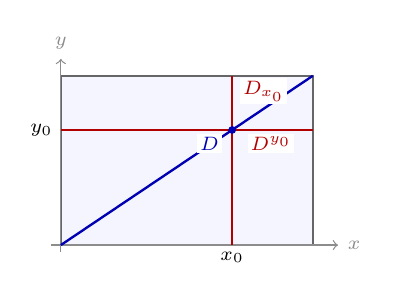
\begin{tikzpicture}[
  x=3.2cm,
  y=2.15cm,
  every node/.style={font=\scriptsize},
  axis/.style={->, black!45, line width=0.45pt},
  square/.style={black!60, line width=0.6pt},
  diagonal/.style={blue!70!black, line width=0.85pt},
  slice/.style={red!70!black, line width=0.65pt},
  labelbox/.style={fill=white, inner sep=1pt}
]
  \draw[square, fill=blue!4] (0,0) rectangle (1,1);
  \draw[axis] (-0.04,0) -- (1.10,0) node[right] {$x$};
  \draw[axis] (0,-0.04) -- (0,1.10) node[above] {$y$};

  \draw[diagonal] (0,0) -- (1,1);
  \node[labelbox, text=blue!70!black, anchor=south west] at (0.54,0.54) {$D$};

  \coordinate (p) at (0.68,0.68);
  \draw[slice] (0.68,0) -- (0.68,1);
  \draw[slice] (0,0.68) -- (1,0.68);
  \fill[blue!70!black] (p) circle[radius=1.4pt];

  \node[labelbox, anchor=north] at (0.68,-0.02) {$x_0$};
  \node[labelbox, anchor=east] at (-0.02,0.68) {$y_0$};
  \node[labelbox, text=red!70!black, anchor=west] at (0.71,0.91) {$D_{x_0}$};
  \node[labelbox, text=red!70!black, anchor=west] at (0.74,0.60) {$D^{y_0}$};
\end{tikzpicture}

  \caption{Diagonal sections: $\nu(D_x)=1$ but $\mu(D^y)=0$.}
  \label{fig:product-diagonal-slices-counterexample}
\end{figure}

\begin{example} \label{ex:double-series-tonelli-fubini-contrast} \hlt{Double Series as Product Integrals}\\
With counting measure on $\N^2$, Tonelli gives, for $a_{mn}\geq0$,\\
$\sum_m\sum_na_{mn}=\sum_{(m,n)\in\N^2}a_{mn}=\sum_n\sum_ma_{mn}\in[0,+\infty]$.\\
Fubini needs integrability: set $a_{nn}=1$, $a_{n,n+1}=-1$, and $a_{mn}=0$ otherwise.\\
Then $\sum_m\sum_na_{mn}=0$, while $\sum_n\sum_ma_{mn}=1$, and $\sum_{m,n}\abs{a_{mn}}=+\infty$.
\end{example}

\begin{proposition} \label{prop:integrable-separated-products} \hlt{Separated Products}\\
Let $(X,\mathcal{M},\mu)$ and $(Y,\mathcal{N},\nu)$ be $\sigma$-finite. If $f\in\mathscr{L}^1(\mu)$, $g\in\mathscr{L}^1(\nu)$, and $H(x,y)\defeq f(x)g(y)$, then $H\in\mathscr{L}^1(\mu\otimes\nu)$ and $\int_{X\times Y}H\,d(\mu\otimes\nu)=(\int_Xf\,d\mu)(\int_Yg\,d\nu)$.
\begin{proof}
Measurability follows from Proposition \ref{prop:product-borel-and-measurable-building-blocks}.\\
Tonelli gives $\int_{X\times Y}\abs{H}\,d(\mu\otimes\nu)=\int_X\abs{f(x)}(\int_Y\abs{g}\,d\nu)d\mu=(\int_X\abs{f}\,d\mu)(\int_Y\abs{g}\,d\nu)<+\infty$, so $H\in\mathscr{L}^1(\mu\otimes\nu)$.\\
Fubini applied to $H$ gives the displayed identity.\\
\hlt{Structural Commentary}: Product-measure integration separates products of one-variable integrable functions.\\
\hlt{Key Insight}: Absolute integrability factors by Tonelli; signed equality follows by Fubini.
\end{proof}
\end{proposition}

\begin{corollary} \label{cor:equal-section-measures-equal-product-measure} \hlt{Equal Section Measures}\\
Let $(X,\mathcal{M},\mu)$ and $(Y,\mathcal{N},\nu)$ be $\sigma$-finite.\\
If $E,F\in\mathcal{M}\otimes\mathcal{N}$ and $\nu(E_x)=\nu(F_x)$ for all $x\in X$, then $(\mu\otimes\nu)(E)=(\mu\otimes\nu)(F)$.
\begin{proof}
Set $f_E(x)\defeq\nu(E_x)$ and $f_F(x)\defeq\nu(F_x)$.\\
Since $f_E=f_F$, Proposition \ref{prop:section-measures-integrate-to-product-measure} gives $(\mu\otimes\nu)(E)=\int_Xf_E\,d\mu=\int_Xf_F\,d\mu=(\mu\otimes\nu)(F)$.\\
\hlt{Structural Commentary}: Product mass is recovered from vertical section masses.\\
\hlt{Key Insight}: Equal fibers give equal product mass.
\end{proof}
\end{corollary}

\begin{definition} \label{def:convolution-real-line} \hlt{Convolution}\\
For Borel $f,g:\R\to\R$, if $y\mapsto f(x-y)g(y)$ is integrable for a.e. $x$,\\
define the \hlt{convolution} $(f*g)(x)\defeq\int_\R f(x-y)g(y)\,dm(y)$ on that full-measure set and $0$ elsewhere.
\end{definition}

\begin{proposition} \label{prop:l1-convolution-basic-bound} \hlt{Convolution of $L^1$ Functions}\\
If Borel $f,g\in\mathscr{L}^1(m)$, then $f*g$ is a.e. defined, $f*g\in\mathscr{L}^1(m)$, and $\int_\R\abs{f*g}\,dm\leq(\int_\R\abs{f}\,dm)(\int_\R\abs{g}\,dm)$.
\begin{proof}
Set $\Phi(x,y)\defeq f(x-y)g(y)$. By Proposition \ref{prop:product-borel-and-measurable-building-blocks}, $\Phi$ is product-measurable.\\
For fixed $y$, translation invariance gives $\int_\R\abs{f(x-y)}\,dm(x)=\int_\R\abs{f}\,dm$.\\
Hence Tonelli yields $\int_{\R^2}\abs{\Phi}\,d(m\otimes m)=(\int_\R\abs{f}\,dm)(\int_\R\abs{g}\,dm)<+\infty$.\\
Fubini gives the a.e. existence of $f*g$, and $\int_\R\abs{f*g}\,dm\leq\int_{\R^2}\abs{\Phi}\,d(m\otimes m)$ gives the bound.\\
\hlt{Structural Commentary}: Convolution is Fubini applied to the difference map $(x,y)\mapsto x-y$.\\
\hlt{Key Insight}: Translation invariance makes every shifted copy of $\abs{f}$ have the same integral.
\end{proof}
\end{proposition}

\begin{example} \label{ex:nonunique-products-without-sigma-finiteness} \hlt{Nonunique Products Without $\sigma$-Finiteness}\\
Let $X=\R$, $\mathcal{M}=2^\R$, and $\mu(A)=0$ if $A$ is countable, $\mu(A)=+\infty$ otherwise.\\
Define $\lambda_i:\mathcal{M}\otimes\mathcal{M}\to\{0,+\infty\}$ by $\lambda_i(E)=0$ exactly on the following null ideals:\\
$\mathcal{I}_1=\{E:E=G\cup H,\ \operatorname{pr}_xG\text{ countable},\ \operatorname{pr}_yH\text{ countable}\}$\\
and $\mathcal{I}_2=\{E:E=G\cup H\cup K,\ \operatorname{pr}_xG\text{ countable},\ \operatorname{pr}_yH\text{ countable},\ \operatorname{pr}_{y=x}K\text{ countable}\}$.\\
Both ideals are closed under countable unions, hence $\lambda_i$ are measures.\\
For every rectangle $A\times B$, both give $\mu(A)\mu(B)$: countable sides are null, and uncountable-by-uncountable rectangles are not in either ideal.\\
For $E=\{(x,y):x+y=0\}$, $\operatorname{pr}_{y=x}E$ is a point, so $\lambda_2(E)=0$ but $\lambda_1(E)=+\infty$.\\
\hlt{Structural Commentary}: Without $\sigma$-finiteness, rectangle values need not determine a product measure.\\
\hlt{Key Insight}: Extra null lines preserve rectangles but change non-rectangles.
\end{example}

\begin{definition} \label{def:lebesgue-product-slices} \hlt{Products and Slices}\\
For $A\subseteq\R^n$, $B\subseteq\R^k$, set $A\times B\subseteq\R^{n+k}$.\\
For $E\subseteq\R^n\times\R^k$ define $E_x\defeq\{y\in\R^k:(x,y)\in E\}$ as \hlt{$x$-slice}, and  $E^y\defeq\{x\in\R^n:(x,y)\in E\}$ as \hlt{$y$-slice}.\\
For $f:E\to\R$, write $f_x(y)=f^y(x)\defeq f(x,y)$ where defined.
\end{definition}

\begin{theorem} \label{thm:measurable-products-product-measure} \hlt{Measurable Products}\\
If $A\subseteq\R^n$, $B\subseteq\R^k$ Lebesgue measurable, then $A\times B$ measurable, $m(A\times B)=m(A)m(B)$; $0\cdot\infty=\infty\cdot0=0$.
\begin{proof}
For boxes $I,J$, $m(I\times J)=m(I)m(J)$; disjoint box decompositions extend this to open sets.\\
First assume $A,B$ are bounded with finite measure.\\
By regularity choose closed $F_A\subseteq A$, $F_B\subseteq B$ and open $G_A\supseteq A$, $G_B\supseteq B$ such that $m(G_A\setminus F_A),\ m(G_B\setminus F_B)<\varepsilon$.\\
Then $F_A\times F_B\subseteq A\times B\subseteq G_A\times G_B$, and the open/closed product formula squeezes $m(A\times B)$ to $m(A)m(B)$.\\
For general $A,B$, set $A_N=A\cap[-N,N]^n$ and $B_N=B\cap[-N,N]^k$. Since $A_N\times B_N\uparrow A\times B$, continuity from below gives $m(A\times B)=\lim_N m(A_N\times B_N)=\lim_N m(A_N)m(B_N)=m(A)m(B)$ with $0\cdot\infty=\infty\cdot0=0$.\\
\hlt{Structural Commentary}: Product measure comes from boxes and regularity.\\
\hlt{Key Insight}: Regularity turns rough measurable products into box products plus zero-set errors.
\end{proof}
\end{theorem}

\begin{theorem} \label{thm:zero-slices-null-set-criterion} \hlt{Zero Slices}\\
If $E\subseteq\R^n\times\R^k$ is Lebesgue measurable, then $E$ is null iff $E_x$ is null for a.e. $x$.
\begin{proof}
\begin{enumerate}[label=\roman*.]
\setlength{\itemsep}{0pt}
\item[$(\Rightarrow)$] If $m(E)=0$, cover $E$ by an open $W$ with small measure.\\
For $X_\alpha(W)=\{x:m(W_x)>\alpha\}$, $m(W)\geq \alpha m(X_\alpha(W))$; letting $m(W)\to0$ gives $m(E_x)=0$ for a.e. $x$.
\item[$(\Leftarrow)$] Remove the exceptional null base so every slice is null. For compact $K\subseteq E$, cover each $K_x$ by a small-measure slice neighborhood; compactness gives finitely many product neighborhoods covering $K$, whose total measure is arbitrarily small by Theorem \ref{thm:measurable-products-product-measure}. Thus $m(K)=0$, hence $m(E)=0$ by regularity.
\end{enumerate}
\hlt{Structural Commentary}: Nullity can be checked fiberwise after removing an exceptional base set.\\
\hlt{Key Insight}: Product measure turns small slice covers into small total measure.
\end{proof}
\end{theorem}

\begin{figure}[H]
  \centering
  \begin{tikzpicture}[
  scale=0.86,
  >=Stealth,
  every node/.style={font=\scriptsize},
  axis/.style={->, black!40, line width=0.5pt},
  boundary/.style={black!75, line width=0.8pt},
  guide/.style={black!22, line width=0.45pt},
  slice/.style={blue!70!black, line width=1pt},
  labelbox/.style={fill=white, inner sep=1pt}
]
  \def\setE{(-2.85,0.45)
    .. controls (-2.55,1.22) and (-1.28,1.44) .. (-0.08,1.40)
    .. controls (1.35,1.36) and (2.78,1.05) .. (3.05,0.20)
    .. controls (3.35,-0.75) and (2.20,-1.45) .. (0.58,-1.55)
    .. controls (-1.10,-1.66) and (-2.55,-1.18) .. (-2.95,-0.28)
    .. controls (-3.08,0.02) and (-3.02,0.25) .. (-2.85,0.45)
    -- cycle}

  \draw[axis] (-3.35,-1.85) -- (3.55,-1.85) node[right] {$x$};
  \draw[axis] (-3.15,-2.05) -- (-3.15,1.85) node[above] {$y$};

  \fill[blue!12] \setE;
  \begin{scope}
    \clip \setE;
    \foreach \x in {-2.2,-1.2,-0.2,0.8,1.8} {
      \draw[guide] (\x,-1.65) -- (\x,1.55);
    }
    \draw[slice] (2.20,-1.23) -- (2.20,0.86);
  \end{scope}
  \draw[boundary] \setE;

  \draw[black!35, line width=0.45pt] (2.20,-1.85) -- (2.20,-1.98);
  \node[labelbox] at (2.20,-2.17) {$x_0$};

  \draw[blue!70!black, line width=0.55pt] (2.20,0.86) -- (2.60,1.12);
  \node[labelbox, text=blue!70!black, anchor=west] at (2.62,1.12) {$E_{x_0}$};
  \node[labelbox] at (-0.30,-1.05) {$E$};
\end{tikzpicture}

  \caption{A planar set can be read by vertical slices; Fubini integrates the slice data over the base variable.}
  \label{fig:cavalieri-slicing-planar-set}
\end{figure}

\begin{theorem} \label{thm:cavalieri-principle-euclidean-slices} \hlt{Cavalieri's Principle for Lebesgue Measure}\\
Let $n,k\in\N$ and $E\in\mathcal{L}^{n+k}$. For $x\in\R^n$ and $y\in\R^k$, set $E_x\defeq\{y:(x,y)\in E\}$ and $E^y\defeq\{x:(x,y)\in E\}$.
\begin{enumerate}[label=(\roman*)]
\setlength{\itemsep}{0pt}
\item $E_x\in\mathcal{L}^k$ for a.e. $x$, and $f_E(x)\defeq m_k(E_x)$ has a measurable representative with $m_{n+k}(E)=\int_{\R^n}f_E\,dm_n$.
\item $E^y\in\mathcal{L}^n$ for a.e. $y$, and $g_E(y)\defeq m_n(E^y)$ has a measurable representative with $m_{n+k}(E)=\int_{\R^k}g_E\,dm_k$.
\end{enumerate}
\begin{proof} Let $\mathsf C_x(E)$ denote: $E_x\in\mathcal L^k$ for a.e. $x$, $f_E$ has a measurable representative, and $m_{n+k}(E)=\int_{\R^n}f_E\,dm_n$.
\begin{enumerate}[label=(\roman*)]
\setlength{\itemsep}{0pt}
\item Rectangles satisfy $\mathsf C_x(A\times B)$ since $f_{A\times B}=m_k(B)\mathbf{1}_A$; finite additivity gives finite unions.\\
For bounded $Q=I\times J$, $\mathcal C_Q\defeq\{E\subseteq Q:\mathsf C_x(E)\}$ is monotone:\\
$E_j\uparrow E$ gives $f_{E_j}\uparrow f_E$ and MCT, while $E_j\downarrow E$ gives $f_{E_j}\downarrow f_E\leq m_k(J)\mathbf{1}_I$ and DCT.\\
Thus $\mathcal C_Q$ contains all Borel $E\subseteq Q$, and exhaustion by $Q_N=[-N,N]^{n+k}$ gives all Borel $E$.\\
For $E\in\mathcal L^{n+k}$, choose Borel $B$ with $m_{n+k}(E\triangle B)=0$; Theorem \ref{thm:zero-slices-null-set-criterion} gives $m_k((E\triangle B)_x)=0$ a.e..\\
Hence $E_x\in\mathcal L^k$ a.e., $f_E=f_B$ a.e., and $m_{n+k}(E)=\int_{\R^n}f_E\,dm_n$.
\item Let $\tau:\R^k\times\R^n\to\R^n\times\R^k$ be $\tau(y,x)=(x,y)$ and put $\widetilde E\defeq\tau^{-1}(E)$.\\
Applying (i) to $\widetilde E\subseteq\R^k\times\R^n$ gives $\widetilde E_y=E^y$ a.e., $g_E(y)=m_n(\widetilde E_y)$, $m_{n+k}(E)=m_{n+k}(\widetilde E)=\int_{\R^k}g_E\,dm_k$.
\end{enumerate}
\hlt{Structural Commentary}: Slices reduce product measure to base integrals.\\
\hlt{Key Insight}: Extend from rectangles, then pass null differences.
\end{proof}
\end{theorem}

\begin{perspective} \label{per:fubini-proof-ladder} \hlt{Fubini Proof Ladder}\\
Fubini ladder: $\mathbf{1}_E\to$ simple $\Phi\geq0\to f\geq0$ by MCT, then $f=f^+-f^-$ when $\int\abs{f}<+\infty$.\\
Theorems \ref{thm:tonelli-sigma-finite-product-measures} and \ref{thm:fubini-sigma-finite-product-measures} are the abstract form.\\
\hlt{Key Insight}: Fubini is a slice theorem, proof runs through indicators, simple functions, monotone convergence.
\end{perspective}

\begin{proposition} \label{prop:undergraph-measurability-level-sets} \hlt{Undergraphs and Level-Set Measurability}\\
Let $f:\R^n\to[0,\infty]$, set $F_a\defeq\{x:f(x)>a\}$, and let $\mathcal{U}f\defeq\{(x,t)\in\R^n\times[0,\infty):0<t<f(x)\}$.
\begin{enumerate}[label=(\roman*)]
\setlength{\itemsep}{0pt}
\item $f$ is Lebesgue measurable iff $F_q\in\mathcal{L}^n$ for every $q\in\Q_{>0}$.
\item If $f$ is Lebesgue measurable, then $\mathcal{U}f\in\mathcal{L}^{n+1}$ and $(\mathcal{U}f)^t=F_t$ for every $t>0$.
\end{enumerate}
\begin{proof}
\begin{enumerate}[label=(\roman*)]
\setlength{\itemsep}{0pt}
\item[$(i)$] ($\Rightarrow$) If $f$ is measurable, each $F_q=f^{-1}((q,+\infty])$ is in $\mathcal L^n$.\\
($\Leftarrow$) If $F_q\in\mathcal L^n$ for all $q\in\Q_{>0}$, then for $a\geq0$, $F_a=\bigcup_{q\in\Q,\ q>a}F_q\in\mathcal L^n$, while for $a<0$, $F_a=\R^n$.\\
Thus all strict superlevel sets are measurable, so $f$ is measurable.
\item[$(ii)$] By (i), every $F_r$ with $r\in\Q_{>0}$ is measurable. Since $\mathcal{U}f=\bigcup_{q,r\in\Q,\ 0<q<r}F_r\times(q,r)$, $\mathcal{U}f\in\mathcal L^{n+1}$.\\
For $t>0$, $(\mathcal{U}f)^t=\{x:0<t<f(x)\}=F_t$.
\end{enumerate}
\hlt{Structural Commentary}: Measurability is encoded by rational superlevels.\\
\hlt{Key Insight}: Undergraph slices are superlevel sets.
\end{proof}
\end{proposition}

\begin{theorem} \label{thm:fubini-tonelli-nonnegative-euclidean} \hlt{Fubini--Tonelli for Nonnegative Functions}\\
Let $f:\R^n\times\R^k\to[0,\infty]$ be Lebesgue measurable.\\
Define $F(x)\defeq\int_{\R^k}f_x\,dm_k$, $f_x$ is measurable and arbitrarily elsewhere; define $G(y)\defeq\int_{\R^n}f^y\,dm_n$ analogously.
\begin{enumerate}[label=(\roman*)]
\setlength{\itemsep}{0pt}
\item $f_x$ is measurable for a.e. $x$, $F$ is measurable, and $\int_{\R^{n+k}}f\,dm_{n+k}=\int_{\R^n}F\,dm_n$.
\item $f^y$ is measurable for a.e. $y$, $G$ is measurable, and $\int_{\R^{n+k}}f\,dm_{n+k}=\int_{\R^k}G\,dm_k$.
\end{enumerate}
\begin{proof}
Put $U\defeq\mathcal{U}f\subseteq\R^{n+k}\times[0,\infty)$. Proposition \ref{prop:undergraph-measurability-level-sets} gives $U\in\mathcal{L}^{n+k+1}$.
\begin{enumerate}[label=(\roman*)]
\setlength{\itemsep}{0pt}
\item By Cavalieri, $U_x$ is measurable for a.e. $x$, $H(x)\defeq m_{k+1}(U_x)$ is measurable, and $m_{n+k+1}(U)=\int_{\R^n}H\,dm_n$.\\
For such $x$, $U_x=\mathcal{U}(f_x)$, so $f_x$ is measurable and $H(x)=\int_{\R^k}f_x\,dm_k=F(x)$.\\
Since $m_{n+k+1}(U)=\int_{\R^{n+k}}f\,dm_{n+k}$, (i) follows.
\item Let $\tau(y,x)=(x,y)$ and $\tilde f\defeq f\circ\tau$.\\
Applying (i) to $\tilde f$ gives $\tilde f_y=f^y$ a.e., $\tilde F=G$, and $\int_{\R^k}G\,dm_k=\int_{\R^{k+n}}\tilde f\,dm_{k+n}=\int_{\R^{n+k}}f\,dm_{n+k}$.
\end{enumerate}
\hlt{Structural Commentary}: Cavalieri applied to the undergraph.\\
\hlt{Key Insight}: $(\mathcal{U}f)_x=\mathcal{U}(f_x)$.
\end{proof}
\end{theorem}

\begin{theorem} \label{thm:fubini-absolutely-integrable-functions} \hlt{Fubini for $L^1$ Functions}\\
Let $f\in L^1(\R^2)$.
\begin{enumerate}[label=(\roman*)]
\setlength{\itemsep}{0pt}
\item $f(x,\cdot)\in L^1(\R)$ for a.e. $x$; defining $F(x)\defeq\int_{\R}f(x,y)\,dy$ there and $F=0$ elsewhere gives $F\in L^1(\R)$.
\item $f(\cdot,y)\in L^1(\R)$ for a.e. $y$; defining $G(y)\defeq\int_{\R}f(x,y)\,dx$ there and $G=0$ elsewhere gives $G\in L^1(\R)$.
\item $\int_{\R}F\,dx=\int_{\R^2}f=\int_{\R}G\,dy$.
\end{enumerate}
\begin{proof}
From Theorems \ref{thm:measurable-products-product-measure}--\ref{thm:zero-slices-null-set-criterion}, the identity holds for indicators.\\
By linearity and MCT, every measurable $h\geq0$ satisfies $(*)\ \int_{\R}(\int_{\R}h(x,y)\,dy)dx=\int_{\R^2}h=\int_{\R}(\int_{\R}h(x,y)\,dx)dy$.
\begin{enumerate}[label=(\roman*)]
\setlength{\itemsep}{0pt}
\item Applying $(*)$ to $\abs f$ gives $\int_{\R}\int_{\R}\abs{f(x,y)}\,dy\,dx=\int_{\R^2}\abs f<+\infty$, so $f(x,\cdot)\in L^1(\R)$ a.e.\\
Let $F^\pm(x)\defeq\int_{\R}f^\pm(x,y)\,dy$; then $F=F^+-F^-$ a.e. and $\int_{\R}\abs F\,dx\leq\int_{\R}(F^++F^-)\,dx=\int_{\R^2}\abs f<+\infty$.
\item Let $\tau(y,x)=(x,y)$ and $\tilde f\defeq f\circ\tau$. Since $\tau$ preserves $m_2$, $\tilde f\in L^1(\R^2)$.\\
Applying (i) to $\tilde f$ gives $\tilde f(y,\cdot)=f(\cdot,y)\in L^1(\R)$ a.e. and $\tilde F=G\in L^1(\R)$.
\item Let $G^\pm(y)\defeq\int_{\R}f^\pm(x,y)\,dx$. By $(*)$, $\int_{\R}F^\pm\,dx=\int_{\R^2}f^\pm=\int_{\R}G^\pm\,dy$. Since these quantities are finite and $F=F^+-F^-$, $G=G^+-G^-$ a.e., subtraction gives $\int_{\R}F\,dx=\int_{\R^2}f=\int_{\R}G\,dy$.
\end{enumerate}
\hlt{Structural Commentary}: Indicators, simple functions, MCT, then $f^\pm$.\\
\hlt{Key Insight}: Absolute integrability permits subtraction.
\end{proof}
\end{theorem}
